\chapter{Clio}

This is only a test.
\section{A section}
Test.

\subsection{A Figure Example}
\label{ssec:figure_example}

This subsection shows a sample figure.

\begin{figure}[h] 
  \centering
  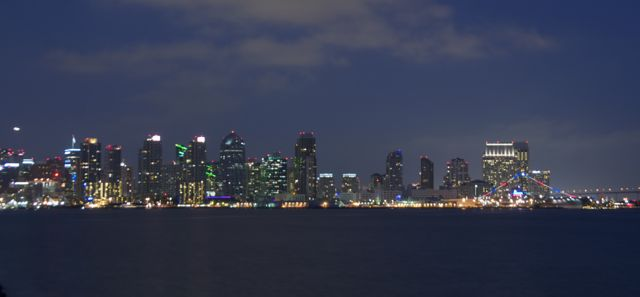
\includegraphics[width=0.5\textwidth]{sandiego}
  \caption[A picture of San Diego. Short figure caption must be \protect{$< 4$} lines in the list of figures]
{A picture of San Diego.  Short figure caption must be \protect{$< 4$} lines in the list of figures and match the start of the main figure caption verbatim. Note that figures must be on their own line (no neighboring text) and captions must be single-spaced and appear \protect\textit{below} the figure.  Captions can be as long as you want, but if they are longer than 4 lines in the list of figures, you must provide a short figure caption.\index{SanDiego}}
  \label{fig:sandiego}
\end{figure}